\section{Methodology}

\begin{figure}[h]
  \centering
  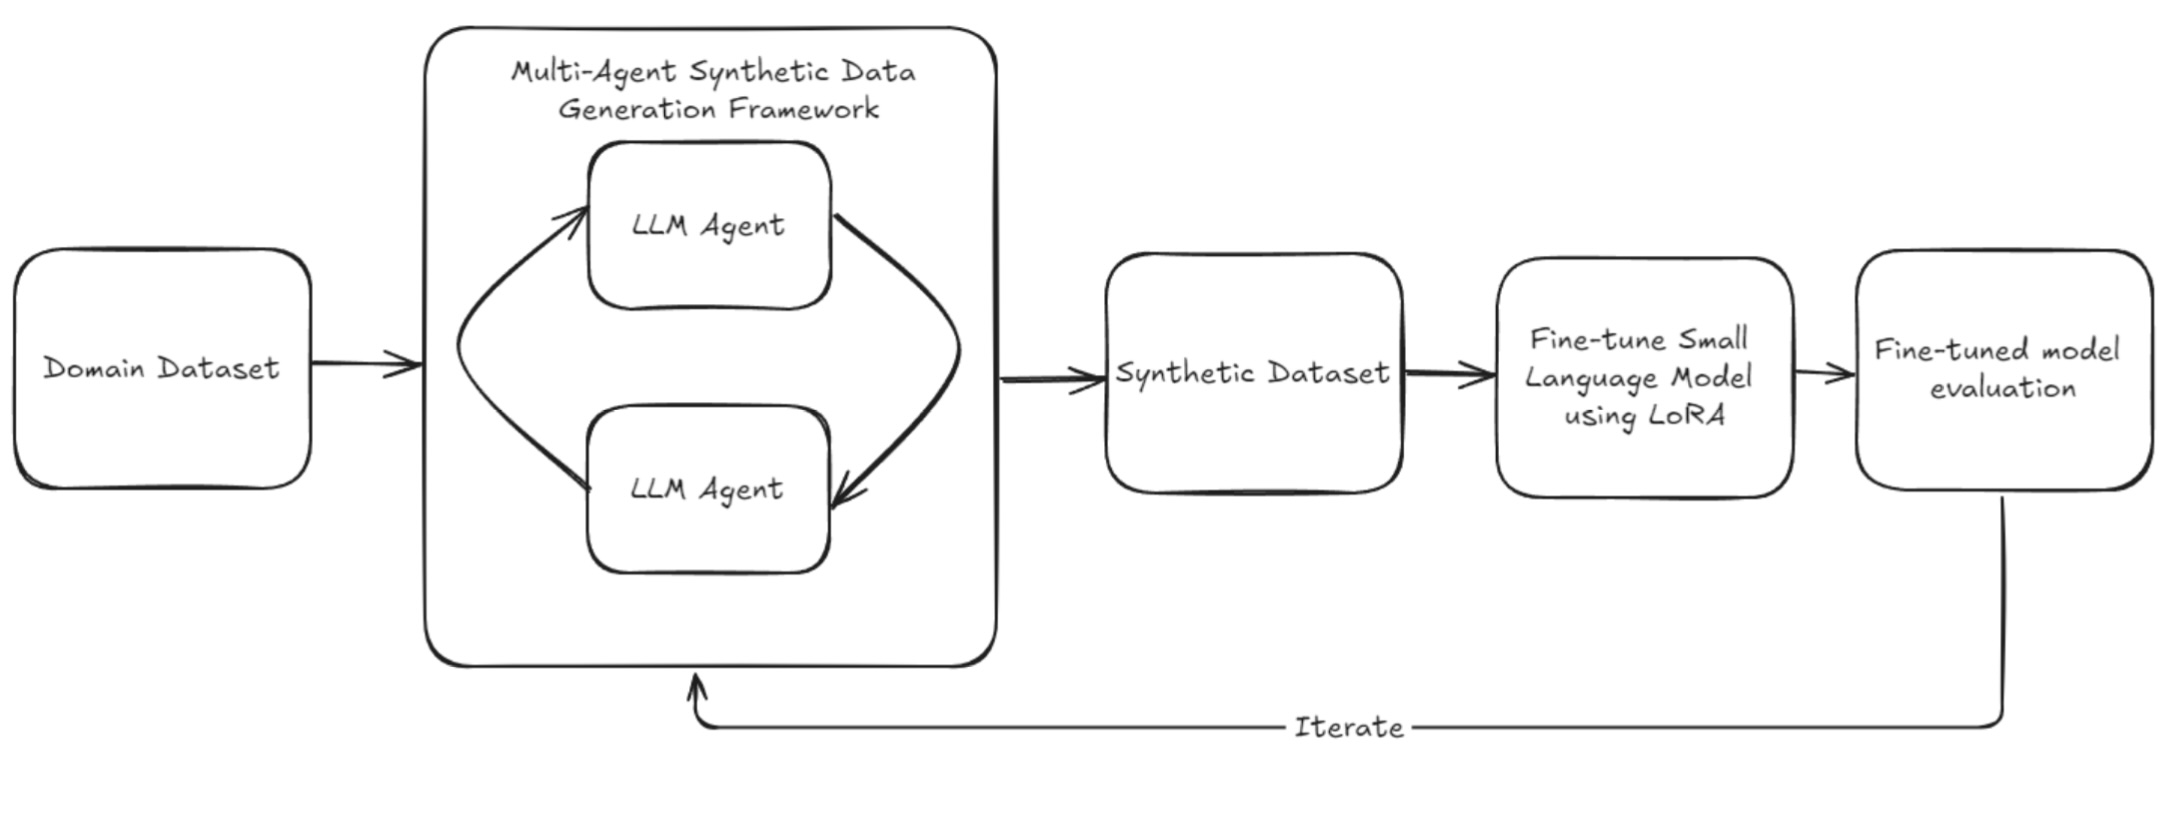
\includegraphics[width=1\textwidth]{methodology.jpg}
  \caption{An overview of our methodology. TODO}
\end{figure}

For our domain datasets that will be used as the seed data, we are still currently exploring datasets that can be used. Current ideas include research papers, company financial data, technical reports and manuals, or company specific FAQ data.
We will develop a multi agent synthetic data generation framework using small language models such as Llama-3.1-8B, Llama-3.2-3B, Qwen2.5-7B to synthetically generate high-quality diverse domain specific data.. Our immediate goal will be to create a framework for specializing in question answering tasks, similar to that of a traditional chatbot. Time permitting, we may expand this scope to also minimize hallucinations from model responses.
Next we will use the data to fine-tune LoRA adapters on the base model chosen. Since this will be an iterative process, we may also choose to perform a full supervised fine-tune of the model depending on resource limitations.

\subsection{Challenges}

One of the challenges we foresee may be overfitting on the fine-tuned model and the models inability to generalize to different writing styles and formats. We plan to mitigate this by increasing the diversity of our generated data. Another challenge is hallucination: previous research has shown that fine-tuning LLMs with new factual information increases their tendency to hallucinate (Gekhman et al. 2024). However, because we consider applications where the questions posed to the LLMs are related to data in the fine-tuning dataset, it's possible that this effect will be reduced (as opposed to questions unrelated to the domain, where a clear effect has already been observed in existing literature).
